%=============================================================================
%=============================================================================

\chapter{Babel-based Interfaces}
\label{ch-babel}

\section{Introduction}

Much of \hypre{} is accessible through a multi-language interface
built through the Babel tool.  This tool can connect to \hypre{} from
your code which you can write in any of several languages.

The Struct (Structured grid), SStruct (Semi-Structured grid), and IJ
(linear algebra style) interfaces all can be used
this way.  The code you write to call \hypre{} functions through the
Babel-based interface works much the same as the code you write to
call them through the original C interface.  The function names are
different, the object structure of \hypre{} is more visible, and there
are many more minor differences.

This chapter will discuss these differences and present brief
examples.  You can also see them in action by looking at the complete
examples in the examples directory.

You do not need to have the Babel software to use the Babel-based
interface of \hypre{}.  Prebuilt interfaces for the C, C++, Fortran,
and Python languages are included with the \hypre{} distribution. We
will enlarge the distribution with more such interfaces whenever
\hypre{} users indicate that they need them, and our tools such as
Babel support them.  Although you do not need to know about Babel to
use the Babel-based interface of \hypre{}, if you are curious about
Babel you can look at its documentation at
\url{http://www.llnl.gov/CASC/components}.

\section{Interfaces Are Similar}
\label{sec-Interfaces-Similar}

In most respects, the older C-only interface and the Babel-based
interface are very similar. The function names always differ a little,
and often there are minor differences in the argument lists.  The
following sections will discuss the more significant differences, but
this example shows how similar the interfaces can be.  The first
example is for the C-only interface, and the other examples are for
the Babel interface in the C, C++, Fortran, and Python languages.

\begin{verbatim}
   HYPRE_IJVectorInitialize( b );
   bHYPRE_IJParCSRVector_Initialize( b, &_ex );
   b.Initialize();
   call bHYPRE_IJParCSRVector_Initialize_f( b, ierr, ex )
   b.Initialize()
\end{verbatim}


\section{Interfaces Are Different}
\label{sec-Interfaces-Different}

Function names usually differ in minor ways, as decribed in the
following section \ref{sec-Names-Conventions}.  But sometimes they
differ more; for example to apply a solver to solve linear equations,
you say \code{Solve} in the C-only interface and \code{Apply} in the
Babel-based interface.  For information on particular functions, see
the reference manuals or example files.

Function argument lists look mainly the same.  The data types of many
arguments are different as required, for example in C a preconditioner
would be a \code{HYPRE_Solver} in the C-only interface, or a
\code{bHYPRE_Solver} in the Babel-based interface.  Sometimes there
are greater differences; the greatest ones are discussed below.
Again, see the reference manuals or example files for more specific
information.

In C or Fortran, the Babel-based interface requires an extra argument
at the end, called the ``exception.''  It is not necessary for C++ or
Python.  You should ignore it, but it has to be there.  In C you
should declare it as follows.
\begin{verbatim}
  #include "sidl_Exception.h"
  sidl_BaseInterface _ex;
\end{verbatim}
And in Fortran you should declare it as follows.
\begin{verbatim}
      integer*8  ex
\end{verbatim}

Parameters are set differently in the C-only and Babel-based
interfaces.  In the C interface there is a different \code{Set}
function for each parameter; the parameter name is part of the
function name.  In the Babel-based interface there are just a few
\code{Set*Parameter} interfaces.  The parameter is one of the
arguments.  For details see section
\ref{sec-Parameters-ErrorFlags}, or look in an example file.

MPI communicators are passed differently, in the native form in the
C-only interface and as a language-neutral object in the Babel-based
interface.  For details see section \ref{sec-MPI}.

In two rare cases, the Babel-based interface of \hypre{} provides
output arrays in a special format.  See section \ref{sec-Arrays}
if you need to deal with it.

With the Babel-based interface in the C or Fortran languages, you will
occasionally need to explicitly cast an object between different data
types.  You do this with a special \code{cast} function.  Moreover,
for every time you create or cast an object you need a corresponding
call of a \code{Destroy} or \code{deleteRef} function. See the
sections \ref{sec-Memory} and \ref{sec-Casting} for details.


\section{Names and Conventions}
\label{sec-Names-Conventions}

In the C-only interface, most \hypre{} function names look like
\code{HYPRE_ClassFunction} where \code{Class} is a class name and
\code{Function} is a (conceptual) function name.  The C-Babel
interface is similar: most function names look like
\code{bHYPRE_Class_Function}.  In the Fortran-Babel interface, most
function names look like \code{bHYPRE_Class_Function_f}.  In the
C++-Babel interface, SIDL (Babel) classes are actually implemented as
classes, so functions generally look like Instance.Function, where
Instance is an instance of the class.  In C++, the
Babel-interface functions live in the namespace \code{::ucxx::bHYPRE}.

This function naming pattern is slightly broken in the case of service
functions provided by Babel rather than \hypre{}.  All of them contain
a double underscore, \code{__}.  These functions are used for casting,
certain arrays, and sometimes memory management.  For more information
see sections \ref{sec-ObjectStructure}, \ref{sec-Arrays}, and
\ref{sec-Memory}.

Most functions are member functions of a class.  In
non-object-oriented languages, the first argument of the function will
be the object which ``owns'' the function.  For example, to solve
equations with a PCG solver you ``apply'' it to vectors using its
member function \code{Apply}.  In C++, C, Fortran, and Python this
concept is expressed as:
\begin{verbatim}
      pcg_solver.Apply( b, x );   (C++;in the ::ucxx::bHYPRE namespace)
      bHYPRE_PCG_Apply( PCG_solver, b, &x, ex );   (C)
      call bHYPRE_PCG_Apply_f( PCG_solver, b, x, ierr, ex )   (Fortran)
      pcg_solver.Apply( b, x )  (Python)
\end{verbatim}

In the Babel interface, data types usually look like \code{Class} in
C++, \code{bHYPRE_Class} in C, and \code{integer*8} in Fortran.  Similar
data types in the C-only interface would look like
\code{HYPRE_Class}.  Here \code{Class} is a class name where the
interface is defined in the SIDL file \code{Interfaces.idl}.
Sometimes the class name is slightly different in the C-only
interface, but usually they are the same.

Most \hypre{} objects need to be supplied with an MPI communicator.
The Babel interface has a special class for the MPI communicator; for
details see section \ref{sec-MPI}.

\section{Parameters and Error Flags}
\label{sec-Parameters-ErrorFlags}

Most \hypre{} objects can be modified by setting parameters.  In the
C-only interface, there is a separate function to set each parameter.
The Babel-based interface has just a few parameter-setting functions
for each object.  The parameters are identified by their names, as
strings.  See below for some examples.

Most \hypre{} functions return error flags, as discussed elsewhere in
this manual. The following examples simply show how they are returned,
not how to handle them.

\subsubsection{C-only}
\begin{verbatim}
    HYPRE_Solver amg_solver;
    int ierr;
    ierr = HYPRE_BoomerAMGSetCoarsenType( amg_solver, 6 );
    ierr = HYPRE_BoomerAMGSetTol( amg_solver, 1e-7 );
\end{verbatim}

\subsubsection{C-Babel}
\begin{verbatim}
    bHYPRE_BoomerAMG amg_solver;
    int ierr;
    ierr = bHYPRE_BoomerAMG_SetIntParameter( amg_solver, "CoarsenType", 6, ex );
    ierr = bHYPRE_BoomerAMG_SetDoubleParameter( amg_solver,
                                                "Tolerance", 1e-7, ex);
\end{verbatim}

\subsubsection{Fortran-Babel}
\begin{verbatim}
          integer*8  amg_solver
          integer ierr
          call bHYPRE_BoomerAMG_SetIntParameter_f(
         1        amg_solver, "CoarsenType", 6, ierr, ex )
          call bHYPRE_BoomerAMG_SetDoubleParameter_f(
         1        amg_solver, "Tolerance", tol, ierr, ex )
\end{verbatim}

\subsubsection{C++-Babel}
\begin{verbatim}
    using namespace ::ucxx::bHYPRE;
    BoomerAMG amg_solver;
    ierr = amg_solver.SetIntParameter( "CoarsenType", 6);
    ierr = amg_solver.SetDoubleParameter( "Tolerance", 1e-7);
\end{verbatim}

\subsubsection{Python-Babel}
\begin{verbatim}
    ierr = solver.SetIntParameter( "CoarsenType", 6 )
    ierr = solver.SetDoubleParameter( "Tolerance", 1e-7 )
\end{verbatim}


\section{MPI Communicator}
\label{sec-MPI}

In the C-only \hypre{} interface, and most normal MPI usage, one often
needs an MPI communicator of type \code{MPI_Comm}.  What an
\code{MPI_Comm} really is depends on the language and the MPI
implementation.

But the Babel interface is supposed to be fundamentally independent of
languages and implementations.  So the MPI communicator is wrapped in
a special \code{bHYPRE_MPICommunicator} object.  This, not an
\code{MPI_Comm} object, is what you pass to all the Babel-interface
functions which need an MPI communicator.  Thus the language
dependence of MPI is isolated in the function which creates the
\code{bHYPRE_MPICommunicator} object.  Here are examples of how to use
this function:

\subsubsection{C-Babel}
\begin{verbatim}
    bHYPRE_MPICommunicator mpi_comm;
    MPI_Comm mpicommworld = MPI_COMM_WORLD;
    MPI_Comm * C_mpi_comm = &mpicommworld;
    mpi_comm = bHYPRE_MPICommunicator_CreateC( C_mpi_comm, ex );
       ...
    parcsr_A = bHYPRE_IJParCSRMatrix_Create( mpi_comm,... );
\end{verbatim}

\subsubsection{C++-Babel}
\begin{verbatim}
    using namespace ::ucxx::bHYPRE;
    MPICommunicator mpi_comm;
    MPI_Comm mpicommworld = MPI_COMM_WORLD;
    MPI_Comm * C_mpi_comm = &mpicommworld;
    mpi_comm = MPICommunicator::CreateC( C_mpi_comm );
       ...
    parcsr_A = IJParCSRMatrix::Create( mpi_comm,... );
\end{verbatim}

\subsubsection{Fortran-Babel}
\begin{verbatim}
          integer*8  mpi_comm
          integer*8  F_mpi_comm
          F_mpi_comm = MPI_COMM_WORLD
          call bHYPRE_MPICommunicator_CreateF_f(F_mpi_comm,mpi_comm,ex)
             ...
          call bHYPRE_IJParCSRMatrix_Create_f( mpi_comm, ... )
\end{verbatim}

\section{Memory Management}
\label{sec-Memory}

You will want to destroy whatever objects you create.  In C and
Fortran, you must do this explicitly.  Through the Babel-based
interface to \hypre{}, there are two ways to create something: by
calling a \code{Create} function or by calling a
\code{cast} function. You can destroy things with a \code{Destroy}
or \code{deleteRef} function.  For every call of \code{Create} or
\code{cast} there must be a call of \code{Destroy} or
\code{deleteRef}.  Here is an example in C:
\begin{verbatim}
    b = bHYPRE_IJParCSRVector_Create( mpi_comm, ilower, iupper, ex );
    vb = bHYPRE_Vector__cast( b, ex );
    bHYPRE_Vector_deleteRef( vb, ex );
    bHYPRE_IJParCSRVector_deleteRef( b, ex );
\end{verbatim}
Here it is in Fortran:
\begin{verbatim}
      call bHYPRE_IJParCSRVector_Create_f( mpi_comm, ilower, iupper,
     1                                     b, ex )
      call bHYPRE_Vector__cast_f( b, vb, ex )
      call bHYPRE_IJParCSRVector_deleteRef_f( vb, ex )
      call bHYPRE_IJParCSRVector_deleteRef_f( b, ex )
\end{verbatim}

What is actually going on here is memory management by reference
counting.  Babel reference-counts all its objects.  Reference
counting means that the object contains an integer which counts the
number of outside references to the object.  Babel will bump up the
reference count by one when you call a \code{Create} or \code{cast}
function.  Note that each of those functions normally is used to
assign an object to a variable.  In C and Fortran it is up to you do
decrement the reference count when that variable is no longer needed.

With Babel, reference counting is automatic in C++, so you will not
normally need to do any memory management yourself.

If you are interested in doing more with reference counting, see the
Babel users' manual for more information.  In some cases you may find
Babel's memory tools useful, e.g. if you copy pointers to Babel
objects.


\section{Casting}
\label{sec-Casting}

If your code is written in C or Fortran, you will occasionally need to
call a Babel \code{cast} function.  This section tells you why and
how.

Functions are generally written in as much generality as possible.
For example, the PCG algorithm works the same for any kind of matrix
and vector, as long as it can multiply a matrix and vector, compute an
inner product, and so forth.  So two of its arguments are of type
\code{bHYPRE_Vector}.  But when you create a vector you have to decide
how it's going to be stored!  So you have to declare it as a more
specific data type, e.g. \code{bHYPRE_StructVector}.  To apply the PCG
solver to that vector in C or Fortran, you have to call a \code{cast}
function to change its data type.

In C++ and Python, you do not normally need to call a \code{cast}
function.

Be careful to call a \code{deleteRef} or \code{Destroy} function to
correspond to every \code{cast} function, as discussed in section
\ref{sec-Memory}.

Here are examples of casting in C and Fortran.
\begin{verbatim}
    bHYPRE_StructVector b_S = bHYPRE_StructVector_Create(...);
    bHYPRE_Vector       b = bHYPRE_Vector__cast( b_S, ex );
    hypre_Vector        x;
    bHYPRE_PCG          PCG_solver;
    bHYPRE_PCG_Apply( PCG_solver, b, &x, ex );
    bHYPRE_Vector_deleteRef( b, ex );
    bHYPRE_StructVector_deleteRef( b_S, ex );
\end{verbatim}
\begin{verbatim}
      integer*8 b_S
      integer*8 b
      integer*8 x
      integer*8 PCG_solver
      call bHYPRE_StructVector_Create_f(...,b_S, ex )
      call bHYPRE_Vector__cast_f( b_S, b, ex )
      call bHYPRE_PCG_Apply_f( PCG_solver, b, x, ierr, ex )
      call bHYPRE_Vector_deleteRef_f( b, ex )
      call bHYPRE_StructVector_deleteRef_f( b_S, ex )
\end{verbatim}
(Other code not shown would set up the matrix, provide it and
parameters to the solver, set up the vectors, and so forth).

\section{The HYPRE Object Structure}
\label{sec-ObjectStructure}

Even though it is written in C, \hypre{} is object-oriented in its
conceptual design.  The object structure of \hypre{} is often visible,
for example in names of structs and functions.  It is even more
visible in the Babel-based interface than in the C-only interface.  In
both interfaces, you can use \hypre{} without any knowledge of its
object structure or object-oriented programming.  This section is for
you if you have some basic knowledge of object-oriented concepts and
if you are curious about how they appear in \hypre{}.

In this section we will touch on some of the more notable features and
peculiarities of the object system as seen through the Babel-based
interface.  It is completely described elsewhere: the object structure
is precisely defined in the a file \code{Interfaces.idl}, written in
SIDL, which is short for ``Scientific Interface Definition Language''.
For more information about the SIDL language, visit the Babel project
website, \url{http://www.llnl.gov/CASC/components}.  For the briefest
possible description of the overall ideas of the \hypre{} object
system, see Figure~\ref{figObjectModel}.

Babel translates this object structure as appropriate for the language
the user uses - from SIDL's interfaces and classes to C++ classes, or
to mangled names in C and Fortran.  For example the
\code{StructVector} class defined in \code{Interfaces.idl} can appear
as a C++ class also named \code{StructVector} (in the \code{bHYPRE}
namespace), as a C struct named \code{bHYPRE_StructVector}, or as a
Fortran \code{integer*8}.  Its member function SetValues can appear in
C++ as a member function \code{SetValues}, in C as a function
\code{bHYPRE_StructVector_SetValues}, or in Fortran as a subroutine
\code{bHYPRE_StructVector_SetValues_f}.

The Babel interface goes beyond the \hypre{} design in that a solver
and matrix are both a kind of operator, i.e. something which acts on a
vector to compute another vector.  If a solver takes a preconditioner,
it is called a preconditioned solver.  There is no class or interface
for preconditioners --- it is possible, though not always wise, to use
any solver as a preconditioner.

In order for a solver to act as an operator, to map a vector to a
vector, it must contain not only a solution method but also the
equations to be solved.  So you supply the solver with a matrix while
constructing the solver.

All solvers have very similar interfaces, so most of their features
are accessible through their common \code{Solver} interface. But each
has its own peculiarities and each takes a different set of
parameters.  Most solvers are specific to one or two matrix classes.
An exception is the four Krylov solvers, which will run with any
matrix.

In contrast to the solvers, matrices have almost nothing in common
other than being operators, i.e. a matrix can multiply a vector to
compute another vector.  Once the storage scheme of the matrix is
specified there is much to do - such as specifying stencils, index
ranges, and grids.  There are four different classes of matrix for
four different storage schemes - ParCSR, structured, and two kinds of
semi-structured matrix.  ParCSR matrices are generally used for
unstructured meshes but do not incorporate the mesh.  A structured
matrix includes a structured grid.  The semistructured matrix classes
share the same interface with minimal modifications, and both contain
mesh information. But their implementations, e.g. matrix storage, are
different.

Conceptually, there can be multiple views, or ways of interfacing, to
a matrix.  Or one type of view can be used for more than one matrix
class.  At present, the Babel interface doesn't contain more than one
view for any matrix class.  For vectors as well the Babel-based
interface is capable of multiple views but no more than one per class
has been implemented.

For each matrix storage method there is a corresponding vector storage
method.  When a matrix class contains a grid or not, so does the
corresponding vector class.  So there are four vector classes just as
there are four matrix classes.  All vector classes inherit from a
common interface to accomodate the common vector operations such as
inner products, sums, and copies.

Here is an example of a full path through the inheritance tree: In the
SIDL file defining the Babel interface, the StructVector class
inherits from the StructVectorView and Vector interfaces.
StructVectorView extends MatrixVectorView interface, which extends the
ProblemDefinition interface.


The inheritance structure matters in use because sometimes you must
cast an object up and down its inheritance hierarchy to provide an
object of the right data type in a function call.  See section
\ref{sec-Casting}.



\begin{figure}
\centering
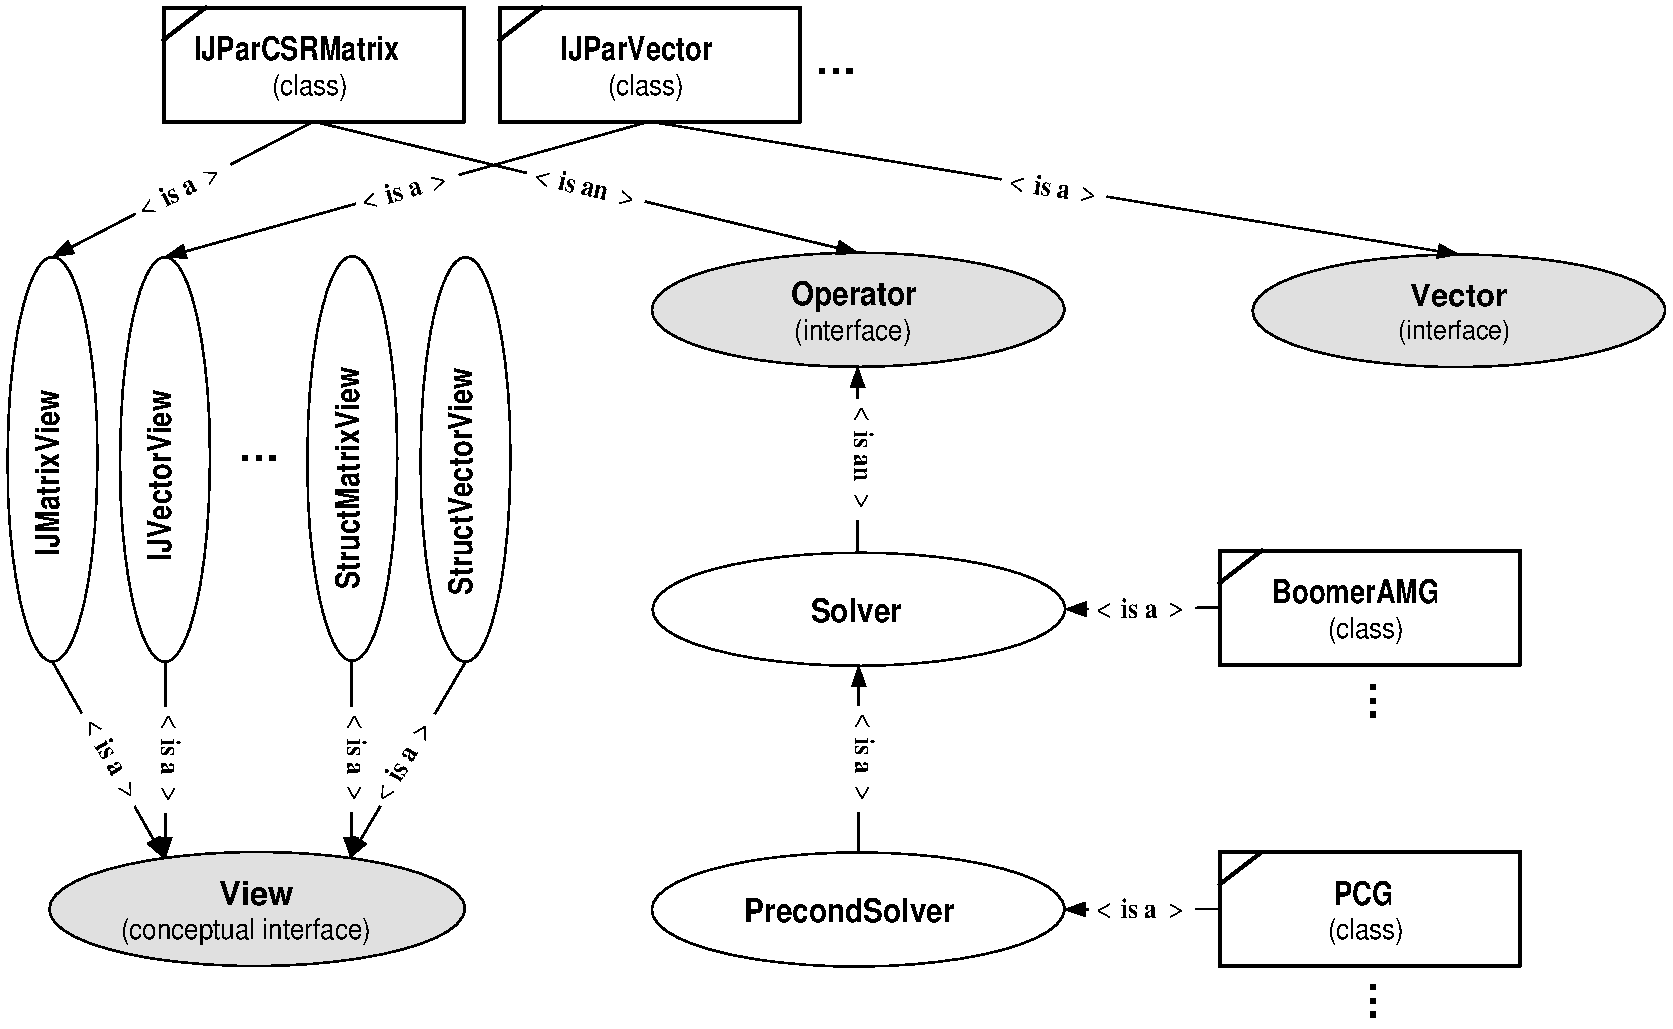
\includegraphics[width=5in]{figObjectModel}
\caption{%
The ideas of the hypre object model.}
\label{figObjectModel}
\end{figure}

% The same chart appears in the following two places, among others.
% 1. page 5 of ``The Design and Implementation of hypre, a Library of
% Parallel High Performance Preconditioners''
% (jfp has this in an email from Rob Falgout on May 13, 2005)
% 2. slide 79 of ACTS viewgraphs on hypre dated August 23, 2005 (jfp
% has this in an email from Rob Falgout dated July 19, 2006)


% >>>>>>> a more complete chart would be nice, if it would fit! <<<<<<<<

% >>>>>>> a verbal description of the object system, e.g. what is a
% view, is ESSENTIAL ! <<<<<<<<<
% concepts to include:
% conceptual interface (e.g. IJ) vs 'underlying storage type' (e.g. ParCSR)

\section{Arrays}
\label{sec-Arrays}

Almost always, when you pass an array through the Babel-based
interface, you do it in the natural way - you build and use the array
type which is native to your language.  Babel calls this kind or array
a ``raw array'' or ``rarray.''  In \hypre{}, they are
one-dimensional too.  It is usually obvious how to use them.

Just two functions in \hypre{}, \code{GetRow} and
\code{CoefficentAccess}, require a special type of array, which Babel
calls a ``SIDL array.''  This has more structure than the arrays
native to languages like C or Fortran - it accomodates reference
counting and knows its own size, for example.

The following examples show a way to declare, read, and destroy a SIDL
array.  The GetRow and CoefficentAccess functions create their output
arrays, so there is no need to create your own.  For more information
on these arrays, read the Babel documentation at
\url{http://www.llnl.gov/CASC/components}.

% I've never done any of this.  This should be put in the test
% programs sometime.

\subsubsection{C}
\begin{verbatim}
    struct sidl_int__array *row_js;
    struct sidl_double__array *row_data;
    bHYPRE_IJParCSRMatrix_GetRow( A, i, &row_size, &row_js, &row_data, ex );
    for ( k=0; k<row_size; ++k )
       col[k]  = sidl_int__array_get1( row_js, k );
       data[k] = sidl_double__array_get1( row_data, k );
    sidl_int__array_deleteRef( row_j, ex );
    sidl_double__array_deleteRef( row_data, ex );
\end{verbatim}
\subsubsection{Fortran}
\begin{verbatim}
      integer*8 row_js;
      integer*8 row_data;
      call bHYPRE_IJParCSRMatrix_GetRow_f( A, i, row_size, row_js,
     1                                     row_data, ex )
      do k = 1, row_size
         call sidl_int__array_get1_f( row_js, k-1, col(k) )
         call sidl_double__array_get1_f( row_data, k-1, data(k) )
      enddo
      call sidl_int__array_deleteRef( row_j, ex )
      call sidl_double__array_deleteRef( row_data, ex )
\end{verbatim}


\section{Building HYPRE with the Babel Interface}
\label{sec-Building-Babel}

You can build \hypre{} almost the same way with and without the
Babel-based interface.  Normally the only difference is that the
configure line needs an extra argument; for example:

\begin{verbatim}
    configure --with-babel
    make
\end{verbatim}
rather than
\begin{verbatim}
    configure
    make
\end{verbatim}

The configure system will enable whatever built-in languages it can
find compilers for.

The configure system for the runtime portion of Babel (included with
\hypre{} and enabled with the Babel-based interface) will
automatically compile and run a few tiny test programs.  This has been
a problem in multiprocessing AIX systems, where compiled programs are
normally run in a different environment from the configure system.
For AIX systems with POE, the
\hypre{} distribution includes a workaround script, \code{nopoe}.
When necessary, build \hypre{} as follows instead of the above:

\begin{verbatim}
    nopoe configure --with-babel
    make
\end{verbatim}

% I could write something about how building interfaces to other
% languages, but that may be too advanced for a user manual.

\subsection{Building HYPRE with Python Using the Babel Interface}
\label{sec-Building-Babel-Python}

To build the hypre library so you can call it from Python code, the
first step is to build a suitable Python!  Start with a recent version
of Python with the Numeric Python extension; for details see the
section on recommended external software in the Babel Users' Manual.

We have only tested hypre's Python interface with pyMPI, a Python
extension which supports MPI.  It is likely that you can make it work
with other MPI extensions, or even no MPI at all.  If you try this,
let us know how it works.

You will need write access to your Python's site-packages directory.
When you install pyMPI it creates another instance of Python, so this
should not be a problem.

You must configure and build hypre with shared libraries, because
Python requires them.  And specify what Python you are building for;
files will be written into its site-packages directory.
For example:
\begin{verbatim}
  configure --with-babel --enable-shared --enable-python=pyMPI
  make
\end{verbatim}

Finally, you need to set two environment variables.
\code{LD_LIBRARY_PATH} must include the path to the hypre shared
libraries, e.g. \code{src/hypre/lib}.
\code{SIDL_DLL_PATH} must include the path to an
\code{.scl} file generated for the Python interface,
e.g.\begin{verbatim}
src/babel/bHYPREClient-P/libbHYPRE.scl
\end{verbatim}
If you are running multiple processes, these environment variables may
need to be set in a dotfile so all processes will use the same values.

See the examples directory for an example of how to write a Python
program which uses hypre.
